\documentclass[crop,tikz]{standalone}% 'crop' is the default for v1.0, before it was 'preview'
\begin{document}
    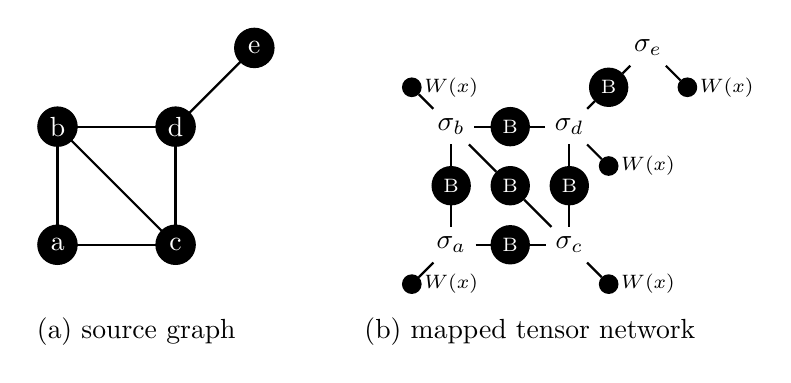
\begin{tikzpicture}[
    dot/.style = {circle, fill, minimum size=#1,
                inner sep=0pt, outer sep=0pt},
    dot/.default = 6pt  % size of the circle diameter 
                    ]  
        \def\dx{0};
        \def\r{0.25cm}
        \filldraw[fill=black] (\dx,0) circle [radius=\r];
        \filldraw[fill=black] (\dx,1.5) circle [radius=\r];
        \filldraw[fill=black] (1.5+\dx,0) circle [radius=\r];
        \filldraw[fill=black] (1.5+\dx,1.5) circle [radius=\r];
        \filldraw[fill=black] (2.5+\dx,2.5) circle [radius=\r];
        \draw [black,thick] (\dx,0) -- (\dx,1.5);
        \draw [black,thick] (\dx,0) -- (1.5+\dx,0);
        \draw [black,thick] (\dx,1.5) -- (1.5+\dx,1.5);
        \draw [black,thick] (1.5+\dx,0) -- (1.5+\dx,1.5);
        \draw [black,thick] (1.5+\dx,0) -- (\dx,1.5);
        \draw [black,thick] (2.5+\dx,2.5) -- (1.5+\dx,1.5);
        \node[color=white] at (\dx,0) {a};
        \node[color=white] at (\dx,1.5) {b};
        \node[color=white] at (1.5+\dx,0) {c};
        \node[color=white] at (1.5+\dx,1.5) {d};
        \node[color=white] at (2.5+\dx,2.5) {e};
        \def\dx{5};
        \def\r{0.25cm}
        \foreach \x/\y/\e in {0.75/0/ac, 0/0.75/ab, 1.5/0.75/cd, 0.75/1.5/bd, 0.75/0.75/bc, 2/2/de}
            \node[color=white,fill=black,dot=2*\r] at (\x+\dx,\y) (\e) {\scriptsize B};
        \foreach \x/\y/\v in {0/0/a, 0/1.5/b, 1.5/0/c, 1.5/1.5/d, 2.5/2.5/e}
            \node[color=black] at (\x+\dx,\y) (\v) {$\sigma_\v$};
        \foreach \x/\y/\v in {-0.5/-0.5/a, -0.5/2.0/b, 2.0/-0.5/c, 2.0/1.0/d, 3.0/2.0/e}
            \node[color=white,fill=black,dot=\r] at (\x+\dx,\y) (\v\v) {};
        \foreach \x/\y/\v in {-0.5/-0.5/a, -0.5/2.0/b, 2.0/-0.5/c, 2.0/1.0/d, 3.0/2.0/e}
            \node[color=black] at (\x+\dx+0.5,\y) {\scriptsize $W(x)$};
        \def\CA{black};
        \def\CB{black};
        \def\CC{black};
        \def\CD{black};
        \def\CE{black};
        \draw [\CA,thick] (a) -- (aa);
        \draw [\CA,thick] (a) -- (ab);
        \draw [\CA,thick] (a) -- (ac);
        \draw [\CB,thick] (b) -- (bb);
        \draw [\CB,thick] (b) -- (ab);
        \draw [\CB,thick] (b) -- (bc);
        \draw [\CB,thick] (b) -- (bd);
        \draw [\CC,thick] (c) -- (cc);
        \draw [\CC,thick] (c) -- (ac);
        \draw [\CC,thick] (c) -- (bc);
        \draw [\CC,thick] (c) -- (cd);
        \draw [\CD,thick] (d) -- (dd);
        \draw [\CD,thick] (d) -- (bd);
        \draw [\CD,thick] (d) -- (de);
        \draw [\CD,thick] (d) -- (cd);
        \draw [\CE,thick] (e) -- (ee);
        \draw [\CE,thick] (e) -- (de);
        \node at (1, -1.1) {(a) source graph};
        \node at (\dx+1, -1.1) {(b) mapped tensor network};
    \end{tikzpicture}
\end{document}
 
